\vspace*{100pt}
\subthesischapter{Realización de los casos de uso}
La realización de los casos de uso en el análisis es una colaboración que describe cómo se lleva a cabo y ejecuta un caso de uso determinado en término de las clases del análisis y de sus objetos en interacción, por lo tanto, se centra en los requisitos funcionales. A continuación se describe el caso de uso de mayor relevancia.
    
\begin{center}
    \begin{table}
        \begin{tabularx}{\textwidth}{|X|X|}
            \hline
            \textbf{Caso de uso:} & Iniciar entrenamiento \\\hline
            \textbf{Actores:}     & Usuario \\\hline
            
            \multicolumn{2}{|X|}{        
            \begin{minipage}[t]{0.925\columnwidth}
                \textbf{Descripción:} \\
                Permite iniciar una rutina de entrenamiento seleccionando entre las modalidades disponibles en el sistema
                \vspace{2pt}
            \end{minipage}} \\\hline
            
            \textbf{Requisitos funcionales asociados:} &  RF10, RF14\\\hline
            \textbf{Precondiciones:} & \begin{itemize}
                                            \item Haber iniciado sesión en el sistema
                                            \item El módulo de comunicación del dispositivo móvil debe estar activado y conectado a la red wifi del pedal
                                            \end{itemize}\\\hline
            \textbf{Poscondiciones:} & Los resultados de la nueva rutina quedarán registrados en el sistema \\\hline
            
            % SECTION 1
            \multicolumn{2}{|X|}{        
            \begin{minipage}[t]{0.925\columnwidth}
                \begin{center}
                    \textbf{Sección principal}
                \end{center}
            \end{minipage}} \\\hline
            
            Acción del actor & Acción del sistema \\\hline
            1. El usuario selecciona la opción de entrenamiento en la vista principal, ver anexo 3. & 2. El sistema muestra la interfaz para la selección de la modalidad. \\\hline
            3. El usuario selecciona la opción que desea:
            \begin{itemize}
                \item Caso <<Modalidad ligero>>: ir al curso alterno <<Modalidad ligero>>
                \item Caso <<Modalidad clínico>>: ir al curso alterno <<Modalidad clínico>>
            \end{itemize} &  \\\hline
            
            % SECTION 2
            \multicolumn{2}{|X|}{        
            \begin{minipage}[t]{0.925\columnwidth}
                \begin{center}
                    \textbf{Sección de cursos alternos}
                \end{center}
            \end{minipage}} \\\hline
            \multicolumn{2}{|X|}{        
            \begin{minipage}[t]{0.925\columnwidth}
                    \textbf{Curso alterno: Modalidad ligero}
            \end{minipage}} \\\hline
            
            Acción del actor & Acción del sistema \\\hline
            
            & 
            1. El sistema construye la interfaz con los parámetros generales de la modalidad seleccionada, ver anexo 3(a). \\\hline
            2. El usuario inserta los valores de distancia y tiempo según la dificultad del entrenamiento que desee y presiona en el botón comenzar fig \ref{}. 
            & 
            3. El sistema muestra la escena de juego correspondiente a la modalidad elegida fig\ref{}. \\ &4. Termina el CU. \\\hline
            
            \multicolumn{2}{|X|}{        
            \begin{minipage}[t]{0.925\columnwidth}
                    \textbf{Curso alterno: Modalidad clínico}
            \end{minipage}} \\\hline
            
            Acción del actor & Acción del sistema \\\hline
                
            & 
            1. El sistema construye la interfaz correspondiente a la sección de calibración, ver anexo 3(c). \\\hline
            \begin{enumerate}
                \item[2.] El usuario presiona en los botones iniciar medición, calcular línea base y calcular MCV siguiendo el protocol médico de calibración.
                \item[3.] El usuario presiona en el botón de modalidad clínico.
            \end{enumerate}
            &
            4. El sistema construye la interfaz con los parámetros generales de la modalidad seleccionada, ver anexo 3(b). \\\hline
            5. El usuario inserta los valores de distancia, tiempo y porciento de MCV según la dificultad del entrenamiento que desee y la calibración obtenida y luego presiona en el botón comenzar. 
            & 
            6. El sistema muestra la escena de juego correspondiente a la modalidad elegida fig\ref{}. \\ &7. Termina el CU. \\\hline
            

            %% ------------------------
            % \multicolumn{2}{|X|}{        
            % \begin{minipage}[t]{0.925\columnwidth}
            %     \begin{center}
            %         \textbf{Prototipo de UI}
            %     \end{center}                    
            % \end{minipage}} \\\hline
            
            % \multicolumn{2}{|X|}{        
            % \begin{minipage}[t]{0.925\columnwidth}
            %     \vspace{5pt}
            %     \begin{minipage}[t]{0.5\columnwidth}
            %         \centering
            %         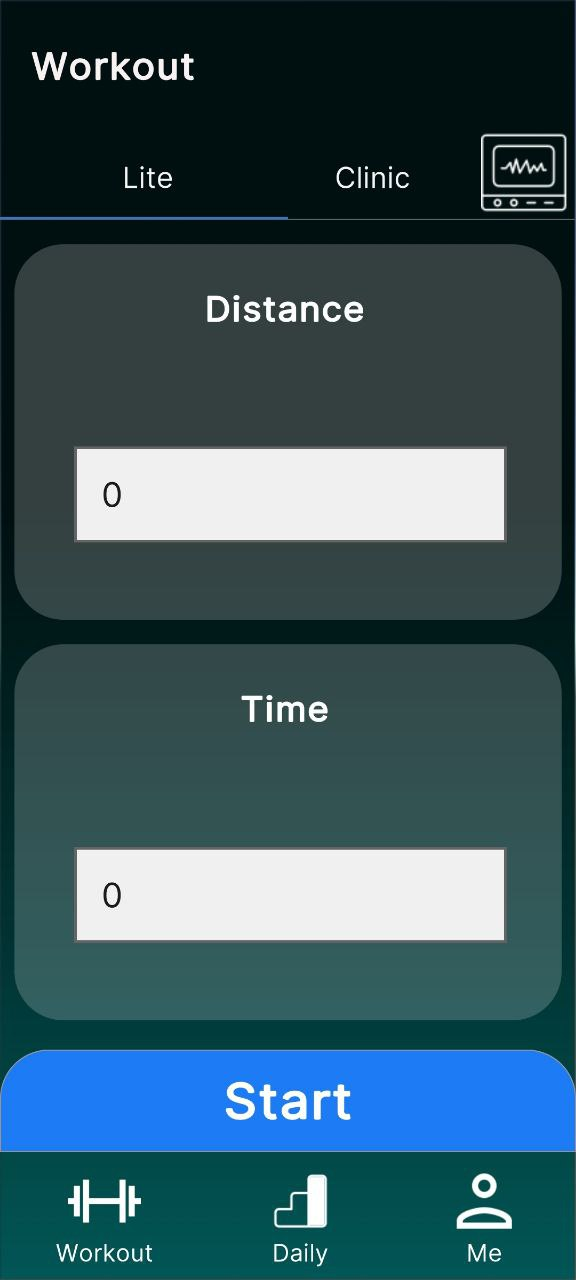
\includegraphics[scale=0.2]{images/ui/2.jpg}
            %         \caption{Pantalla principal}
            %         \label{display: 1}
            %     \end{minipage}
            % \end{minipage}} \\\hline
            


        \end{tabularx}

        \caption{Descripción del CU: Iniciar entrenamiento}
    \end{table}
\end{center}